\documentclass[12pt]{article}
\usepackage[utf8]{inputenc}
\usepackage[top=0.75in, bottom=0.75in, left=0.75in, right=0.75in, headheight=15pt]{geometry}
\usepackage{amsmath, amssymb, amsthm, graphicx, hyperref, enumerate, multirow,  multicol, tikz, centernot, cancel, forest, lipsum, mathtools, bm, esvect, fancyhdr, esdiff, float, parskip, comment}

\DeclareMathSymbol{*}{\mathbin}{symbols}{"01} % change * to /cdot inside math
% \begingroup % let only this align, etc. break across pages
% \allowdisplaybreaks
% \begin{align}
%     ....
% \end{align}
% \endgroup

% \begin{figure}[H]
%     \centering
%     \includegraphics{}
%     \caption{}
%     \label{fig:}
% \end{figure}

% \texorpdfstring{$k$}{k} math inside (sub/)section label

\pagestyle{fancy}
\fancyhead[L]{Liheng Cao}
% \fancyhead[C]{center}
\fancyhead[R]{}

\title{} % title
\author{Liheng Cao} % name
\date{\today} % custom date else today's date

\begin{document}
\maketitle

\section{}
\begin{enumerate}
	\item [Matrix A]
	\begin{enumerate}[(a)]
		\item \[ \lambda_1 = 4, \lambda_2 = -2, v_1 = (1,1), v_2 = (-1,1)\]
		
		\item \[ 1+1 = 1+1 = 2 \]
		
		\item \[ 4*-2 = -8 \]
		
		\item \[ \arccos\left(\dfrac{\langle(1,1),(-1,1)\rangle}{\sqrt{1+1}*\sqrt{1+1}}\right) = \arccos\left(0\right) = \pi/2 \]
		
		\item The eigenvalues are real. The matrix is symmetric.
	\end{enumerate}

	\item [Matrix B]
	\begin{enumerate}[(a)]
		\item \[ \lambda_1 = 37, \lambda_2 = -15, v_1 = (3,2), v_2 = (-2,3)\]
		
		\item \[ 37-15 = 21+1 = 22 \]
		
		\item \[ 37*-15 = -555 \]
		
		\item \[ \arccos\left(\dfrac{\langle(3,2),(-2,3)\rangle}{\sqrt{3^2+2^2}*\sqrt{3^2+2^2}}\right) = \arccos\left(0\right) = \pi/2 \]
		
		\item The eigenvalues are real. The matrix is symmetric.
	\end{enumerate}

	\item [Matrix C]
	\begin{enumerate}[(a)]
		\item \[ \lambda_1 = -1, \lambda_2 = 1, \lambda_3 = 1, v_1 = (-1,0,1), v_2 = (1,0,1), v_3 = (0,1,0)\]
		
		\item \[ -1+1+1 = 0+1+0 = 1 \]
		
		\item \[ -1*1*1 = -1 \]
		
		\item Find the inner products. $ \langle v_1, v_2 \rangle = \langle v_2, v_3 \rangle = \langle v_1, v_3 \rangle = 0 $. Since the inner products are all 0, then the angle is $ \pi/2 $
		
		\item The eigenvalues are real. The matrix is symmetric.
	\end{enumerate}

	\item [(f)]
	Given that $ X $ has all real values, $ X = X^T \implies \operatorname{Im}(v_i) = 0$ 
\end{enumerate}
\newpage

\section{}
\[ \theta = \arccos\left(\dfrac{\langle v, w\rangle}{\|v\| \|w\|}\right) \]

\[ \mathit{PQ} = (2,1,0,3) - (1,2,0,1) = (1,-1,0,2) \]
\[ \mathit{PR} = (0,1,1,0) - (1,2,0,1) = (-1,-1,1,-1) \]
\[ \mathit{RQ} = (2,1,0,3) - (0,1,1,0) = (2,0,-1,3) \]

As long as we take the acute angle, it doesn't matter if a vector is backwards: \textit{PQ}, \textit{QP} are equivalent.

\[ \textit{P} = \arccos\left(\dfrac{\langle \mathit{PQ}, \mathit{PR}\rangle}{\|\mathit{PQ}\| \|\mathit{PR}\|}\right) = 114.095^{\circ}\]

\[ \textit{Q} = \arccos\left(\dfrac{\langle \mathit{PQ},\mathit{RQ}\rangle}{\|\mathit{PQ}\| \|\mathit{RQ}\|}\right) = 29.206^{\circ}\]

\[ \textit{R} = 180-\arccos\left(\dfrac{\langle\mathit{PR},\mathit{RQ}\rangle}{\|\mathit{PR}\| \|\mathit{RQ}\|}\right) = 36.700^{\circ}\]

The 3 sum to $ 180^{\circ} $.
\newpage

\section{}
\begin{align*}
	\langle \vec{N}, \vec{X}-P\rangle &= 0\\
	\langle\vec{N}, \vec{X} \rangle - \langle \vec{N}, P\rangle &= 0\\
	(a_1x_1 + \cdots + a_nx_n) - (r_1x_1 + \cdots + c_nx_n) &= 0 \tag{solves means evals to $b$}\\
	b - b &= 0
\end{align*}
\newpage

\section{}
\[ \theta = \arccos\left(\dfrac{\langle (1,1,1,1), (2,1,3,7)\rangle}{\sqrt{1 + 1 + 1 + 1}*\sqrt{2^2 + 1 + 3^2 + 7^2}}\right) = 35.023^{\circ} \]
\newpage

\section{}
\[ \theta = \arccos\left(\dfrac{\langle (1,1,1,1), (2,3,0,5)\rangle}{\sqrt{1 + 1 + 1 + 1}*\sqrt{2^2+3^2+0+5^2}}\right) = 35.800^{\circ} \]
\newpage

\section{}
\begin{enumerate}[(a)]
	\item \,
	\begin{figure}[H]
		\centering
		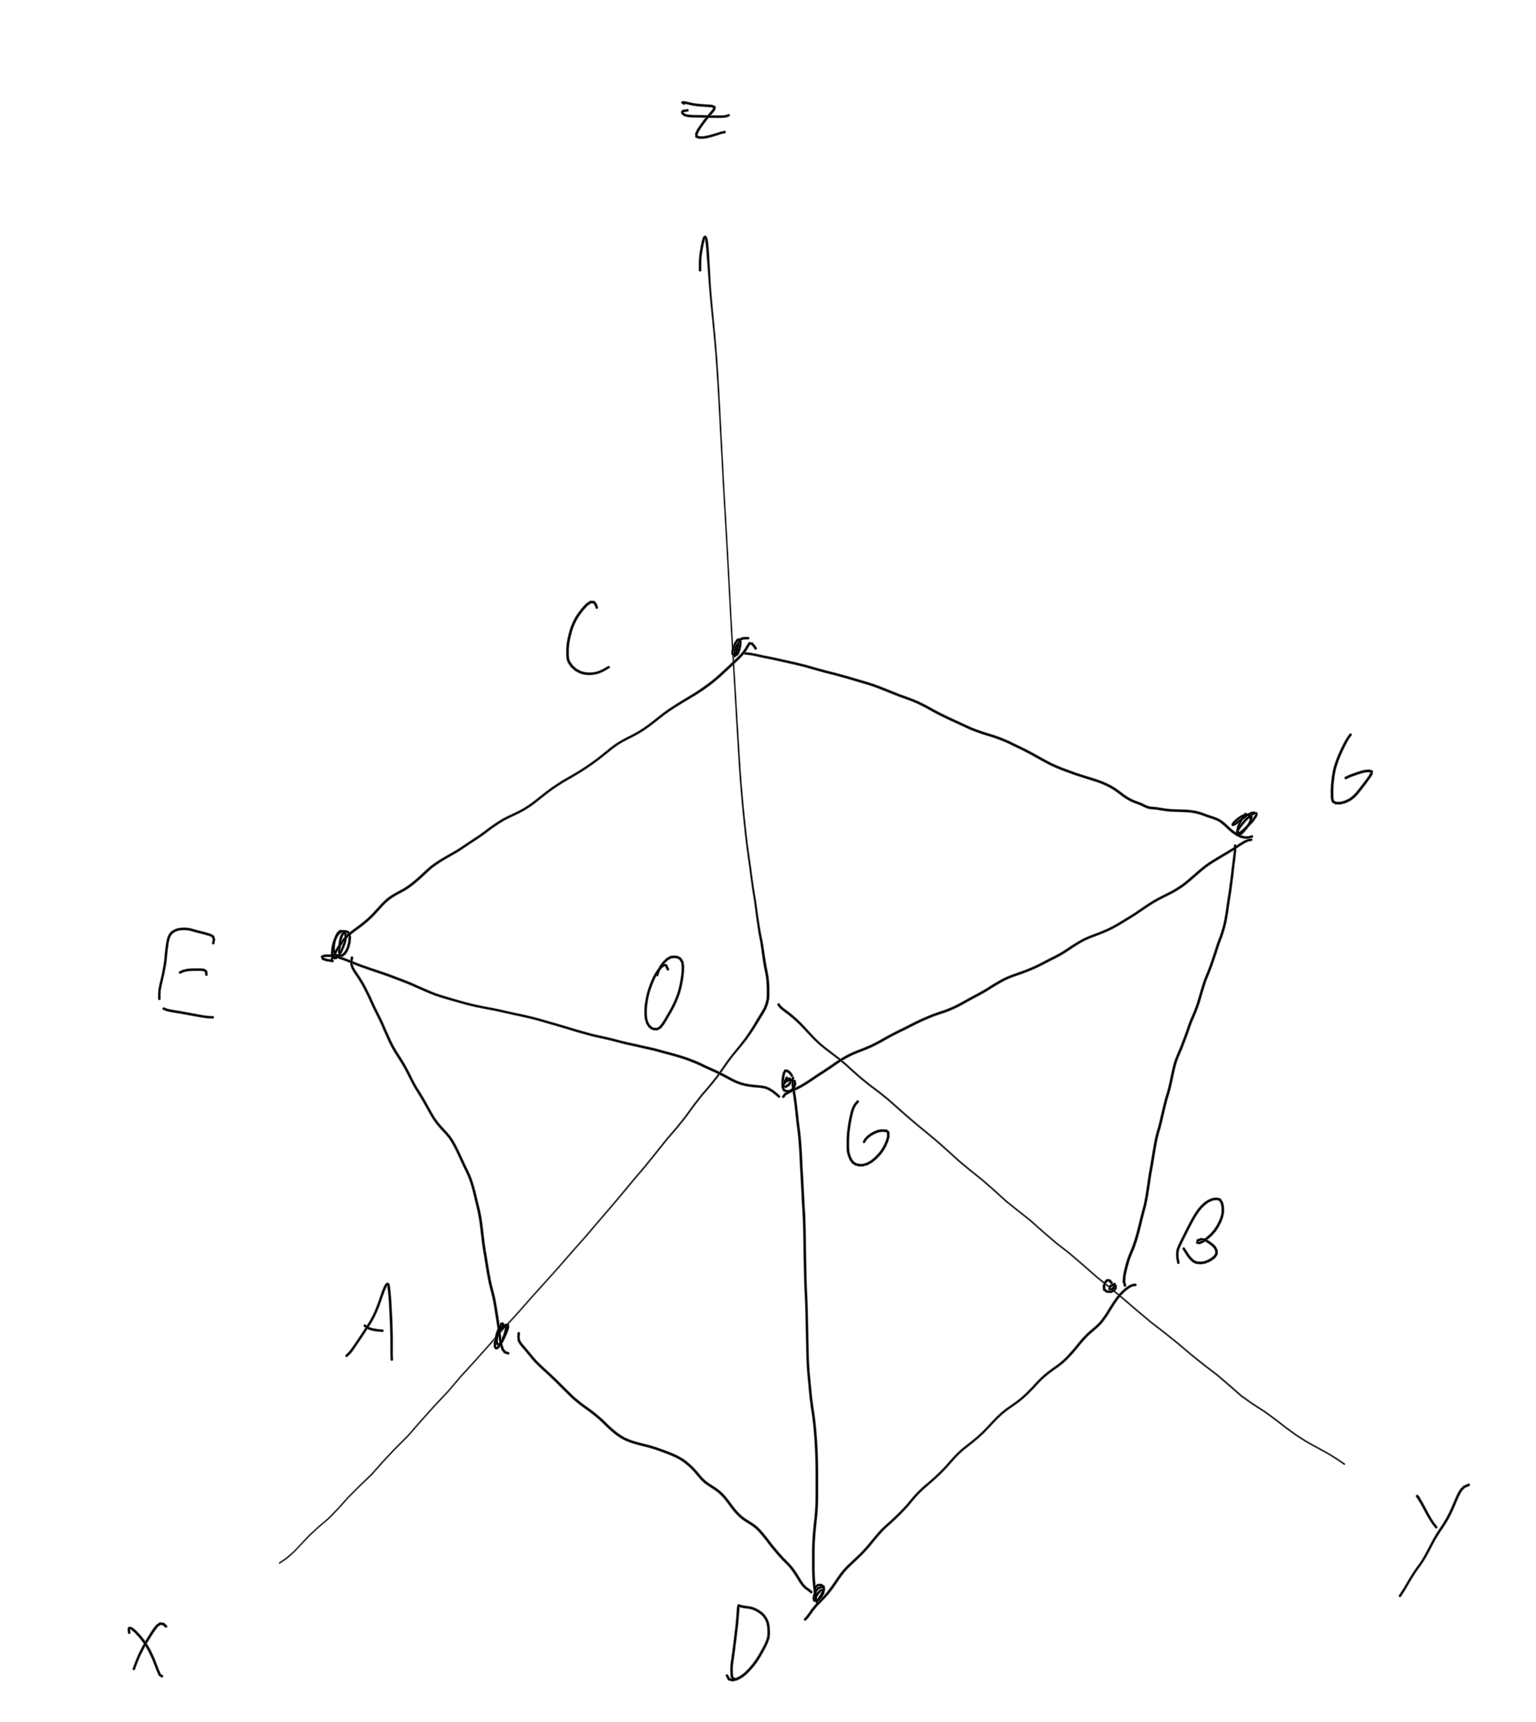
\includegraphics[width=\textwidth]{images/cube.png}
		\caption{rough sketch}
		\label{fig:a:sketch}
	\end{figure}

	\item \[ \sqrt{1+1+1} = \sqrt{3} \]
	
	\item \[ \arccos\left(\dfrac{\langle (1,0,0), (1,1,1)\rangle}{\sqrt{1} * \sqrt{3}}\right) = 54.736^{\circ}\]
\end{enumerate}
\newpage

\section{}
\begin{enumerate}[(a)]
	\item \[ \|x^2\| = \sqrt{\langle x^2, x^2 \rangle} = \sqrt{\int_{0}^{1} x^2 * x^2 \,dx} = \sqrt{1/5}\]
	\[ \|x^3\| = \sqrt{\langle x^3, x^3 \rangle} = \sqrt{\int_{0}^{1} x^3 * x^3 \,dx} = \sqrt{1/7}\]
	\[\theta = \arccos\left(\dfrac{\langle x^2, x^3 \rangle}{\sqrt{1/35}}\right) = \arccos\left(\dfrac{\int_{0}^{1} x^2 x^3 \,dx}{\sqrt{1/35}}\right) = 9.594^{\circ}\]
	
	\item \[ \|\sin(m\pi x)\| = \sqrt{\langle \sin(m\pi x), \sin(m\pi x) \rangle} = \sqrt{\int_{0}^{1} \sin(m\pi x)\sin(m\pi x)\, dx} = \dfrac{1}{2} - \dfrac{\sin(2m\pi )}{4\pi^2}\]
	
	\[ \|\sin(n\pi x)\| = \sqrt{\langle \sin(n\pi x), \sin(n\pi x) \rangle} = \sqrt{\int_{0}^{1} \sin(n\pi x)\sin(n\pi x)\, dx} = \dfrac{1}{2} - \dfrac{\sin(2n\pi )}{4\pi^2}\]
	
	\[\theta = \arccos\left(\dfrac{\langle \sin(m\pi x), \sin(n\pi x)\rangle}{\left(\dfrac{1}{2} - \dfrac{\sin(2n\pi )}{4\pi^2}\right)\left(\dfrac{1}{2} - \dfrac{\sin(2m\pi )}{4\pi^2}\right)}\right) = \arccos\left(\dfrac{\int_0^1 \sin(m\pi x)\sin(n\pi x)\,dx}{den}\right)\]
	
	If $ m=n $, then the angle between something that is itself would be 0. 
\end{enumerate}
\newpage

\section{}
\begin{enumerate}[(a)]
	\item We get $ I_4 $. This tell us that the rows are independent.
	
	\item We get \[\begin{bmatrix}
		1 & 0 &-1 & 0 & 1\\
		0 & 1 & 2 & 0 & -2\\
		0 & 0 & 0 & 1 & 2\\
		0 & 0 & 0 & 0 & 0\\
		0 & 0 & 0 & 0 & 0
	\end{bmatrix}\] Since we have 2 rows of all 0, this means they are dependent. We would need to add $ (0,0,1,0,0), (0,0,0,0,1) $ because the third and fifth column do not have a leading 1.

	\item We get \[\begin{bmatrix}
		1 & 0 & 0 & 1\\
		0 & 1 & 0 & -3\\
		0 & 0 & 1 & 3\\
		0 & 0 & 0 & 0
	\end{bmatrix}\] Since we have a row of all 0, this means they are dependent. We would need to add $ (0,0,0,1) $ because the fourth column does not have a leading 1.
\end{enumerate}
\newpage

\section{}
Use the hint. \[ \sum_{k=1}^{n} a_k \langle w_j, w_k \rangle = 0\] can be simplified into \[a_k \langle w_j, w_k \rangle = 0\] because $ j \neq k \implies \langle w_j, w_k \rangle = 0 $. Only one pair $ j = k $ evaluates to $ 1 $, so \[a_k = 0\] We can vary $ j $ to get that every $ a_k = 0 $.
\newpage

\section{}
\begin{enumerate}[(a)]
	\item \[ \operatorname{Proj}_v(w) = \dfrac{\langle (1,2,0,0,1), (1,1,1,0,1) \rangle }{1+4+1} * (1,2,0,0,1) = \dfrac{1+2+1}{6} * (1,2,0,0,1) = (2/3, 4/3, 0, 0, 2/3) \] In this case, $ \lambda = 2/3 $
	
	\item \[ w = (\lambda * v) + (w-\lambda * v) \]
	\[(1,1,1,0,1) = [2/3 (1,2,0,0,1)] + [(1,1,1,0,1)-2/3(1,2,0,0,1)]\]
	\[\langle v, w - \lambda * v\rangle = 0\]
	\[\langle (1,2,0,0,1), (1,1,1,0,1)-2/3(1,2,0,0,1)\rangle = 1 - 2/3 + 2- 8/3 + 1 - 2/3 = 0\]
\end{enumerate}
\newpage

\section{}
\[ v = \{(1,2,0,1), (0,1,1,4), (1,1,1,1) \} \]
\begin{align*}
	v_1 &= \dfrac{(1,2,0,1)}{\sqrt{1+4+1}}\\
	w_1 &= \dfrac{1}{\sqrt{6}} (1,2,0,1)
\end{align*}
\begin{align*}
	r_2 &= (0,1,1,4) - \langle (0,1,1,4), 1/\sqrt{6}(1,2,0,1)\rangle 1/\sqrt{6} (1,2,0,1)\\
	&= (0,1,1,4) - (2+4)1/\sqrt{6} * 1/\sqrt{6} (1,2,0,1)\\
	&= (0,1,1,4) - 6/6 (1,2,0,1)\\
	&= (-1,-1,1,3)\\
	w_2 &= \dfrac{(-1,-1,1,3)}{\sqrt{1+1+1+9}}\\
	w_2 &= \dfrac{(-1,-1,1,3)}{2\sqrt{3}}
\end{align*}
\begin{align*}
	r_3 &= (1,1,1,1) - \langle (1,1,1,1), 1/\sqrt{6}(1,2,0,1) \rangle 1/\sqrt{6} (1,2,0,1)  (-1,-1,1,3) -\langle v_3, w_2 \rangle w_2 \\
	&= (1,1,1,1) - (4/\sqrt{6})/\sqrt{6} (1,2,0,1) -\langle v_3, w_2 \rangle w_2\\
	&= (1,1,1,1) - 2/3(1,2,0,1) - \langle v_3, w_2 \rangle w_2\\
	&= 1/3 (1, -1, 3, 1) - \langle v_3, w_2 \rangle w_2\\
	&= 1/3 (1, -1, 3, 1) - \langle (1,1,1,1), 1/(2\sqrt{3}) (-1, -1, 1,3) \rangle 1/(2\sqrt{3})(-1,-1,1,3)\\
	&= 1/3 (1, -1, 3, 1) - 1/(2\sqrt{3}) (-1-1+ 1+3) 1/(2\sqrt{3})(-1,-1,1,3)\\
	&= 1/3 (1, -1, 3, 1) - 1/12 * (2) (-1,-1,1,3)\\
	&= 1/6 (3, -1, 5, -1)\\
	w_3 &= \dfrac{(3, -1, 5, -1)}{\sqrt{9+1+25+1}}\\
	w_3 &= 1/6 (3, -1, 5, -1)
\end{align*}
\[ w = \left\{\dfrac{(1,2,0,1)}{\sqrt{6}},\dfrac{(-1,-1,1,3)}{2\sqrt{3}},\dfrac{(3, -1, 5, -1)}{6} \right\} \]

\end{document}